\chapter{Use Cases}
\label{ch:use}

%%%%%%%%%%%%%%%%%%%%%%%%%%%%%%%%


\section{ProtoDUNE II data: acquisition and reconstruction}\label{sec:use:pdii}

Figure \ref{fig:ch:use:pdii} shows the data flow for regular reconstruction.  

\subsection{DAQ to Raw Data store}
The DAQ/CISC systems are expected to provide in close to real time:

\begin{itemize}
    \item The Raw Data
    \item Information on run and trigger configuration
    \item Information on detector conditions
    \item Low level calibration constants such as gains that do not need extensive offline processing
    
\end{itemize}

The raw data is written to disk locally and then copied to the archive site (FNAL). Once the data are confirmed to be on tape, the local copy may be deleted.
A second copy of the raw data should be stored in a different archive. 

The run and trigger information, conditions and calibration constants are made available through separate data paths and stored in appropriate databases.  

\subsection{Raw data to reconstructed hits}

This step takes the raw waveforms, applies  basic channel-to-channel calibrations, removes noise and stuck bits and performs 2D deconvolution.   This processing step operates on large data arrays and may be suitable for different architectures than conventional pattern recognition. It is anticipated that this step will not need to be done frequently. 

\subsection{Hits to Calibration}

In this step, the processed hits from calibration samples are run through specialized pattern recognition and used to derive high quality calibration constants which are stored in a database for future use.   This step will likely be done many times, especially at experiment start.

\subsection{Hits to reconstructed interactions }
In this step, the improved calibration constants and raw hits are input to the full  pattern recognition and reconstructed interactions are output. Data quality can be monitored as part of this processing and stored. 

\subsection{Interactions to Analysis}
The interaction data, which is in the output format supplied by the full reconstruction is reduced and reconfigured into analysis formats for use by users. 

\subsection{Analysis}
Analysis samples should be small and useful.  Analysis should not need to read from the central databases but may access small local replicas. 


\begin{dunefigure}
[Data flow diagram for standard PD reconstruction]
{fig:ch:use:pdii}
{Data flow diagram for standard PD data reconstruction.}
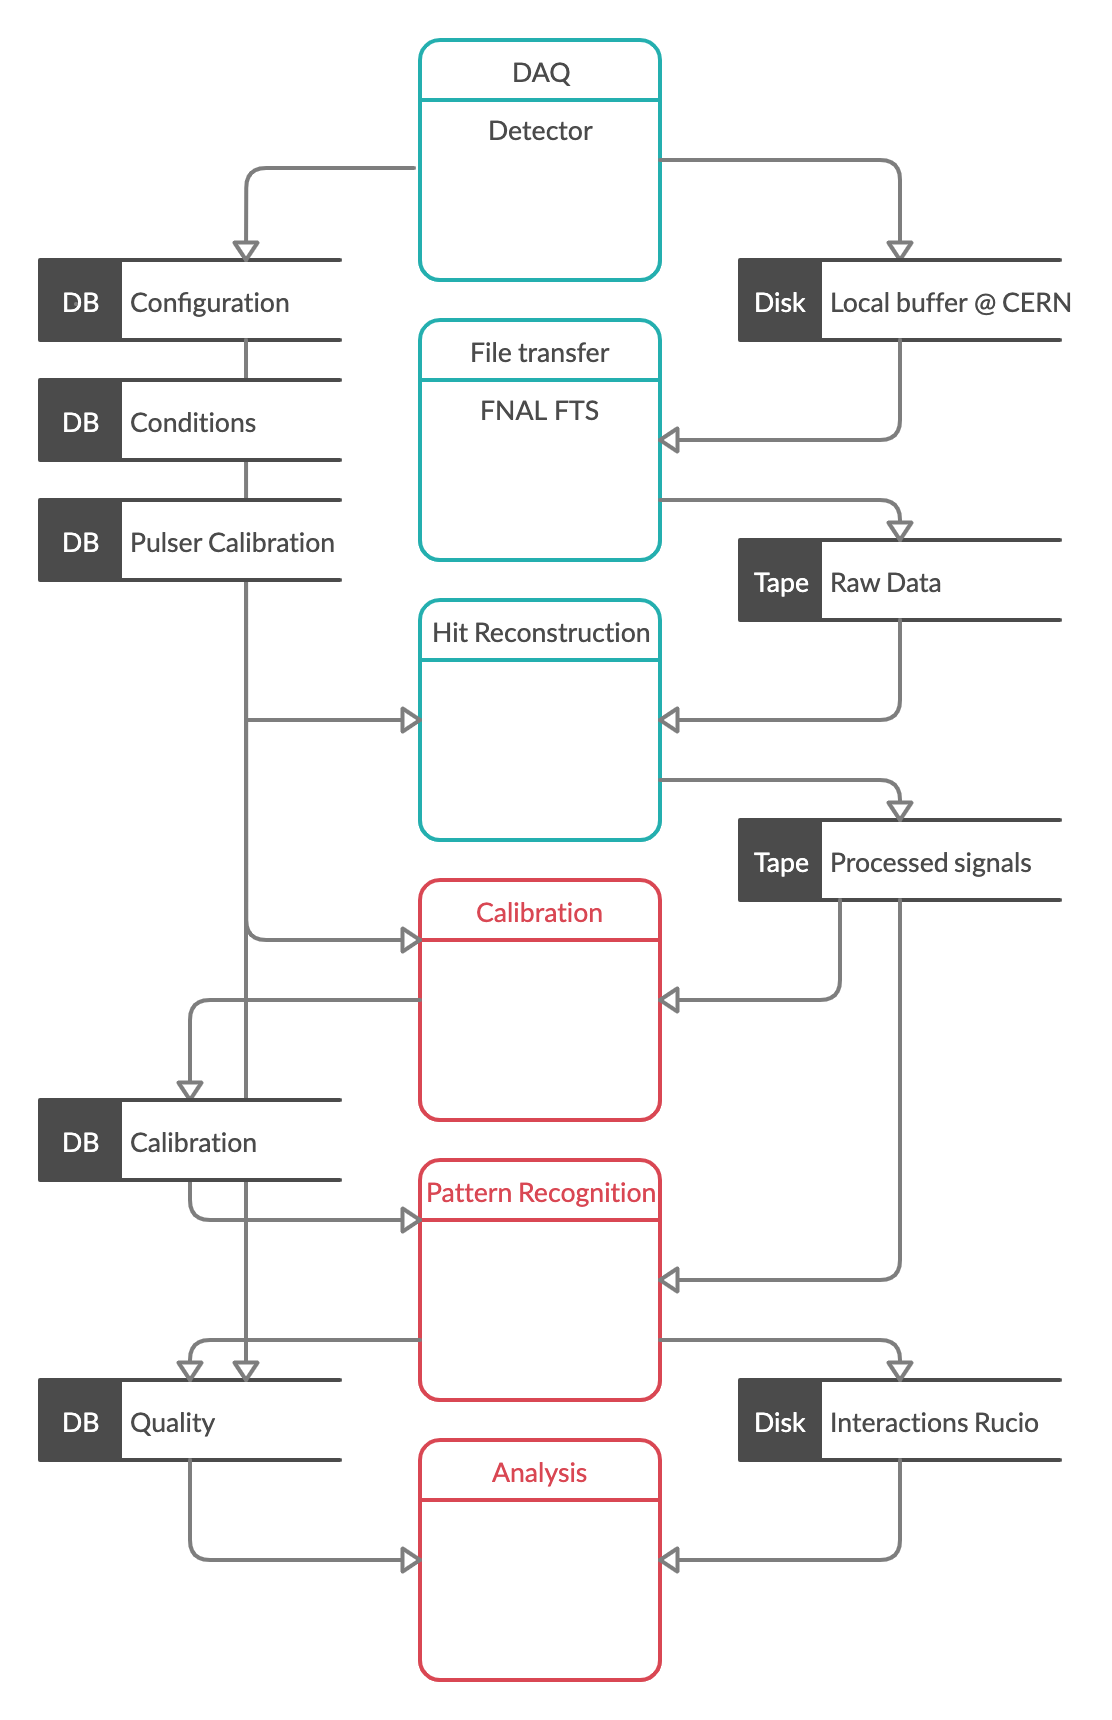
\includegraphics[width=0.8\textwidth]{graphics/IntroFigures/Data processing - PD - v1.png}
\end{dunefigure}
\pagebreak


\section{Data reduction at FNAL before writing it out?}

\section{Fast processing for data monitoring} 

\section{Normal FD readout: FD acquisition and reconstruction}
\label{sec:use:fdbeam}  %% fix label according to section

\section{Beam Data: ND acquisition and reconstruction}
\label{sec:use:ndbeam}  %% fix label according to section

\section{Simulation}  \fixme{Mathews' diagram} 

\section{Oscillation analysis} Chris Backhouse?  Chris Marshall? 
\label{sec:use:osc}

\section{Supernova data: acquisition and fast reconstruction}
\label{sec:use:supernova}  %% fix label according to section

\subsection{Fast ( 1 day turnaround)} \fixme{Priority for readout?}

\subsection{Full Supernova}

\section{Solar/BSM analysis}
\label{sec:use:BSManalysis}

\section{Calibration data: acquisition, reconstruction and use}
\label{sec:use:calib}  %% fix label according to section

\section{Hardware database use case} \fixme{Paul has an example}
\label{sec:use:hdb} 

\section{What's missing?}
\label{sec:use:todo}






